\section{Command and Motion Changes Relative to a Clean Rerun}
\label{sec:supp-matched-motion}
How large is a perturbation's effect on commands and motion, measured against a clean rerun? Under Sensor Noise, $\pi_0$ changes its first five commands and its end-effector position after five controls less than a clean rerun does, yet loses 14.29 points of success; under Camera, both policies end up further from their clean runs after 60 controls than a rerun does (Table~\ref{tab:supp-matched-motion}). This supports Sec.~\ref*{M-sec:sensitivity} of the main paper: the size of a change is not its cost. Section~\ref{sec:early-late-association} shows that command changes reach the robot.

\paragraph{The motion ratio is a ratio of task-equal means.}
Let $R_0,R_1$ be the clean runs with policy-noise draws 0 and 1, $T_0,T_1$ the perturbed runs with the same draws, and $R'_0$ a repeat of $R_0$ (main paper, Fig.~\ref*{M-fig:model-measurement}d). $TR$ is the mean of the two perturbed--clean distances and $RR$ the clean-rerun distance. Both are averaged within tasks, then over tasks equally; we report $TR-RR$ and the ratio of task means $\overline{TR}/\overline{RR}$, below one when the perturbation changes less than a clean rerun. Unlike a mean of per-setting ratios, this ratio is not dominated by settings with a near-zero rerun distance; a zero $RR$ leaves it undefined. A setting enters only if both perturbed--clean distances and the clean-rerun distance are measured in the same record (per policy, family, metric and control step), so numerator and denominator use the same settings. The repeat ($R_0$ vs.\ $R'_0$) and the two perturbed runs ($T_0$ vs.\ $T_1$) form separate panels with their own supports.

\paragraph{Missing outcomes are bounded, not imputed.}
The paired executions (Sec.~\ref{sec:five-arm}) plan 268 settings for each of $\pi_{0.5}$ and $\pi_0$. All 536 policy--setting records exist, but 25 runs failed technically and 14 further outcomes failed validation. These 39 outcomes stay unknown in the fixed denominator of 2,680 runs. Rather than impute them, we report \emph{bounds over missing outcomes}: the lowest and highest value an estimate can take over every assignment of success or failure to the unknown runs. A bound describes missing data, not sampling noise, which is reported separately. The primary scope is the 202 difficulty-labelled settings on the 28 common tasks per policy; all 268 settings form a sensitivity scope. For $\pi_{0.5}$ Light, the primary success change lies between 0 and $+8.04$ percentage points ($-2.92$ to $+5.21$ over all 268 settings); for $\pi_0$ Light it lies between $-2.68$ and $+5.36$ on the primary scope.

\paragraph{Measurements.}
The 15 metrics listed in advance are: the RMS differences of the first five commands (translation, rotation, gripper); end-effector position distance and orientation angle at controls 0/5/15/30/60; and two quantities at each run's own last step. The main paper's motion ratio uses position after five controls. Commands are in command units, positions in meters and orientations in radians. A fixed-time comparison uses only the pose stored at that control step.

\begin{table*}[t]
\caption{\textbf{Relative to a clean rerun, Camera moves the end effector further after 60 controls in both policies, while several families change the commands less than a rerun does.} B, C, L, S: Background, Camera, Light, Sensor Noise. Columns: $TR-RR$ and the ratio of task means $TR/RR$ for the first five commands (translation, command units) and for end-effector (EEF) position after control 60 (meters). $TR$, $RR$: perturbed--clean and clean-rerun distance. Joint $N$/tasks: settings with all three distances measured in the same record. Brackets: pointwise 95\% intervals from paired whole-task draws on the support shown. Each of the 720 comparisons listed in advance keeps its own measured support.}

\centering\footnotesize
\setlength{\tabcolsep}{2.4pt}
\begin{tabular}{@{}llrcccc@{}}
\toprule
Policy & Family & \shortstack{Joint\\$N$/tasks} & \shortstack{Commands\\$TR-RR$} & \shortstack{Commands\\$TR/RR$} & \shortstack{EEF at control 60\\$TR-RR$ (m)} & \shortstack{EEF at control 60\\$TR/RR$}\\
\midrule
$\pi_{0.5}$ & B & 48/28 & $-0.0038[-0.0165,0.0083]$ & $0.91[0.66,1.24]$ & $0.00524[-0.000006,0.01041]$ & $1.27[0.9997,1.65]$\\
$\pi_{0.5}$ & C & 51/28 & $0.0572[0.0359,0.0806]$ & $2.36[1.80,3.04]$ & $0.02281[0.01480,0.03160]$ & $2.29[1.74,3.03]$\\
$\pi_{0.5}$ & L & 43/26 & $-0.0208[-0.0314,-0.0109]$ & $0.52[0.38,0.71]$ & $-0.00104[-0.00598,0.00326]$ & $0.94[0.72,1.24]$\\
$\pi_{0.5}$ & S & 55/28 & $0.0115[-0.0050,0.0281]$ & $1.27[0.90,1.76]$ & $0.01298[0.00519,0.02091]$ & $1.77[1.26,2.48]$\\
\midrule
$\pi_0$ & B & 48/28 & $-0.0343[-0.0535,-0.0159]$ & $0.58[0.43,0.77]$ & $-0.00594[-0.01769,0.00569]$ & $0.83[0.57,1.20]$\\
$\pi_0$ & C & 51/28 & $-0.0017[-0.0212,0.0181]$ & $0.98[0.77,1.27]$ & $0.01924[0.00128,0.04139]$ & $1.55[1.04,2.27]$\\
$\pi_0$ & L & 44/27 & $-0.0619[-0.0799,-0.0452]$ & $0.24[0.17,0.35]$ & $-0.01855[-0.02842,-0.00915]$ & $0.48[0.36,0.67]$\\
$\pi_0$ & S & 55/28 & $-0.0373[-0.0551,-0.0204]$ & $0.55[0.39,0.72]$ & $-0.00120[-0.01258,0.00978]$ & $0.97[0.70,1.34]$\\
\bottomrule
\end{tabular}

\label{tab:supp-matched-motion}
\end{table*}

\paragraph{$\pi_0$ under Sensor Noise moves less than a clean rerun and still loses success.}
For $\pi_0$ under Sensor Noise, the ratio to the clean rerun is $0.545[0.395,0.718]$ for the first five commands and $0.580[0.409,0.791]$ for end-effector position after control 5, while its primary success change is $-14.29$ percentage points. A family mean below the rerun level thus accompanies a net loss of success on the same settings. The position ratios after control 5 (main paper, Table~\ref*{M-tab:outcomes}) are 0.93 (Background), 2.68 (Camera), 0.57 (Light) and 1.32 (Sensor Noise) for $\pi_{0.5}$, and 0.62, 1.03, 0.24 and 0.58 for $\pi_0$. After control 60, Camera ratios exceed one in both policies, which also lose net success under Camera; this sets a distance at a fixed step against an outcome at the episode's end. For $\pi_{0.5}$ Background the ratio after control 60 is $1.273[0.9997,1.6505]$, and the interval of its paired difference spans zero. Light's motion support is 43/48 settings on 26/28 tasks for $\pi_{0.5}$ and 44/48 on 27/28 for $\pi_0$.

\paragraph{Individual pairs against their own clean rerun.}
We also compare each perturbed pair of $\pi_0$ under Sensor Noise (primary scope) with the clean-rerun distance of its own setting. After control 5, let $d_{vn}$ be the end-effector position distance between $T_n$ and $R_n$ for setting $v$ and noise draw $n$, and let $r_v$ be the distance between that setting's $R_0$ and $R_1$. Each recorded pair is classed by $d_{vn}<r_v$, $d_{vn}=r_v$ or $d_{vn}>r_v$, and all four outcome groups are kept (Table~\ref{tab:sensor-case-reference}).

Most pairs that lose a success moved less than a clean rerun: of the 18 lost-success pairs, 12 have $d_{vn}<r_v$. All 55 settings on 28 tasks have both perturbed pairs, measured distances after control 5, a positive clean-rerun distance and known outcomes. The twelve pairs cover ten settings and eight tasks; all lost-success pairs cover fifteen settings and ten tasks. In every setting with a lost-success pair, both clean runs succeed, so the clean rerun changes no outcome there. The two pairs of a setting share one rerun distance, so the counts are nested within settings; they are a descriptive split, while the task-weighted estimates above keep the hierarchy.

\paragraph{Motion size is a poor predictor of lost success (post hoc AUROC).}
The main paper summarizes these pairs by a post hoc AUROC. The score is the ratio $d_{vn}/r_v$; the 18 lost-success pairs are the positive class and the 84 joint-success pairs the negative class, pooled without weights, with ties counted as one half. The AUROC is $0.49$, close to chance. Its 95\% interval, $[0.29,0.70]$, is the percentile interval of 2{,}000 whole-task bootstrap draws that resample the 28 tasks with replacement and keep all pairs of a task together, so the two pairs of a setting keep their shared $r_v$. Every draw contained both classes. With families pooled, the raw distance gives $0.73$ ($\pi_{0.5}$) and $0.64$ ($\pi_0$), and the norm of the change in the first five commands at the first query gives $0.74$ and $0.64$; comparing pairs only within their family gives $0.62\ [0.48,0.74]$ and $0.55\ [0.35,0.70]$ for the ratio. Section~\ref{sec:five-arm} gives the values per family.

\par\medskip\noindent\begin{minipage}{\columnwidth}
\centering\small
\begin{tabular}{lrrrr}\toprule
Outcome & $d<r$ & $d=r$ & $d>r$ & Total\\\midrule
SS: both succeed & 65 & 0 & 19 & 84\\
SF: lost success & 12 & 0 & 6 & 18\\
FS: gained success & 2 & 0 & 0 & 2\\
FF: both fail & 4 & 0 & 2 & 6\\
\midrule
All pairs & 83 & 0 & 27 & 110\\
\bottomrule\end{tabular}
\captionof{table}{\textbf{Pairs that lose a success and pairs that keep it both mostly move less than a clean rerun.} Counts for all 110 $\pi_0$ Sensor Noise pairs (55 settings on 28 tasks). Rows: outcome of the clean and the perturbed run (S, success; F, failure). Columns: whether the pair's end-effector position distance $d_{vn}$ after control 5 is below, equal to or above its own setting's clean-rerun distance $r_v$, which the two pairs of a setting share. All distances and outcomes are available, and all 55 rerun distances are positive.}
\label{tab:sensor-case-reference}
\end{minipage}\par\medskip



\paragraph{Details.}
The comparisons above are part of 720 listed in advance (two policies $\times$ two scopes $\times$ four families $\times$ fifteen metrics $\times$ three references). All are kept: 36 have no joint support and 684 have measured joint support. Each reports its exclusions, tasks, number of paired whole-task draws (2,000) and the reasons for undefined values. The 39 unknown outcomes enter the bounds on success change and on changed outcomes over the planned denominator; motion means use the measured joint support, and the SF/SS groups are post hoc. A zero command distance between $R_0$ and its repeat $R'_0$ leaves that ratio undefined. Final poses are compared only when two runs end at the same control step, which is rare, so they form a separate, sparse comparison from control 60.

\begin{figure*}[p]
\centering
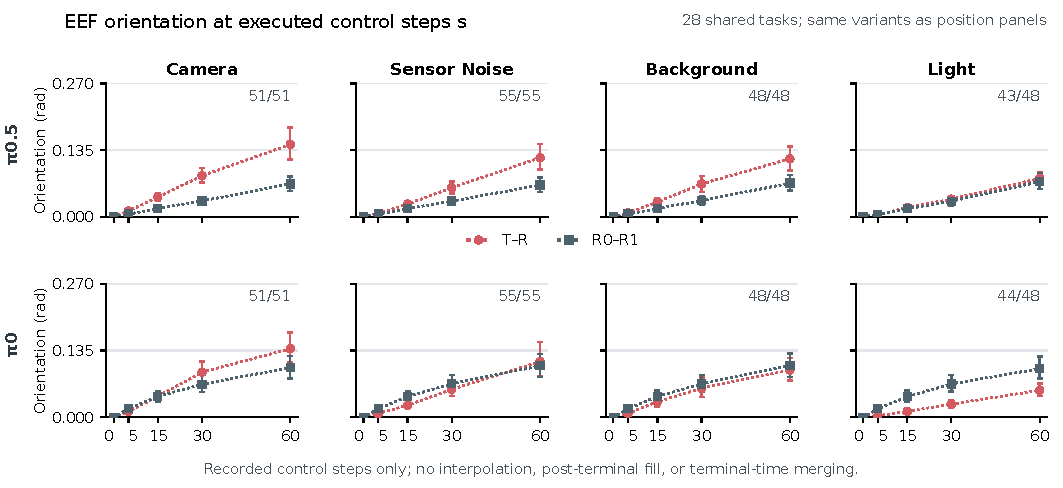
\includegraphics[width=\textwidth]{figures/v77_motion_rotation.pdf}
\caption{\textbf{End-effector orientation, a separate motion endpoint.} Perturbed--clean orientation distances in radians, with the same rule as the position panels (same setting, same control step); each control step has its own joint support. Lines connect the stored measurements; the two policies are shown in separate panels.}
\label{fig:supp-motion-rotation}
\end{figure*}
\clearpage

\subsection{Command changes reach the robot: strongly after 5 controls, still after 60}
\label{sec:early-late-association}
Do changes in the first five commands show in the robot's motion? The command change ranks with end-effector separation almost perfectly after five controls, as expected since those controls execute the commands, and more weakly but clearly after 60 (Table~\ref{tab:early-late-association}; Fig.~\ref{fig:supp-early-late}). This supports Sec.~\ref*{M-sec:early} of the main paper. The comparison uses all 268 planned settings.

\paragraph{Same pairs, two control steps.}
We match the same policy, setting and noise draw after controls 5 and 60, requiring the same first-query command-change norm and a valid end-effector separation at both steps; every outcome group is included. The matched support is 516/536 pairs for $\pi_{0.5}$ and 526/536 for $\pi_0$, each on 40 tasks; unavailable measurements stay counted on the planned support.

\paragraph{Task-weighted rank correlation.}
Each eligible pair has weight $w_{tvn}=1/(T V_t N_{tv})$, weighting tasks, their settings and their noise draws equally at each level. For a scalar $z$, define the weighted midpoint empirical CDF
\begin{equation}
F_w(z_i)=\sum_{j:z_j<z_i}w_j+\tfrac12\sum_{j:z_j=z_i}w_j.
\end{equation}
The rank correlation is the weighted Pearson correlation of these transforms of command-change norm and end-effector distance, pooled over the plotted families with equal task weight. Section~\ref{sec:supp-bounded-internal} instead centers ranks within tasks. Constant tasks stay included; zero overall variance would leave the statistic undefined.

\begin{table}[h]
\caption{\textbf{The command change ranks with end-effector separation more strongly after control 5 than after control 60, in both policies.} Weighted rank correlation on the same pairs at both steps. Brackets are pointwise 95\% intervals for each policy and contrast.}
\centering\small
\begin{tabular}{lrrr}\toprule
Policy & Control 5 & Control 60 & Early minus late\\\midrule
$\pi_{0.5}$ & \shortstack{0.953\\{[0.933,0.968]}} & \shortstack{0.474\\{[0.362,0.580]}} & \shortstack{0.479\\{[0.368,0.593]}}\\
$\pi_0$ & \shortstack{0.974\\{[0.961,0.982]}} & \shortstack{0.409\\{[0.303,0.512]}} & \shortstack{0.566\\{[0.463,0.671]}}\\
\bottomrule\end{tabular}

\label{tab:early-late-association}
\end{table}

\paragraph{Uncertainty and units.}
The analysis rules were fixed before these calculations, on data already observed. Intervals come from 10,000 whole-task bootstrap draws, shared by both control steps, with the weighted CDFs recomputed in each draw; percentile intervals use linear interpolation, and all draws are defined. Command norms use the fifteen translation coordinates (command units); end-effector distances are in millimetres.

